\documentclass[12pt,a4paper]{report}
\usepackage[top=1in, bottom=1in, left=1.5in, right=1in]{geometry}
\usepackage{times}
\usepackage{graphicx}
\usepackage{amsmath}
\usepackage{amssymb}
\usepackage{booktabs}
\usepackage{multirow}
\usepackage{array}
\usepackage{caption}
\usepackage{subcaption}
\usepackage{float}
\usepackage{setspace}
\usepackage{fancyhdr}
\usepackage{hyperref}
\usepackage{microtype}
\usepackage{titlesec}

% Change "Contents" to "CONTENTS OF SYNOPSIS" and format the TOC
\renewcommand{\contentsname}{\centering CONTENTS OF SYNOPSIS}

% Format section titles
\titleformat{\section}[block]{\normalfont\Large\bfseries\centering}{\thesection.}{0.5em}{}

% Redefine section numbering to just be 1, 2, 3 instead of 0.1, 0.2 (since we removed chapters)
\renewcommand{\thesection}{\arabic{section}}

\tolerance=1000
\emergencystretch=3em

\onehalfspacing

\pagestyle{fancy}
\fancyhf{}
\fancyfoot[L]{\thepage\ $|$ \small FBS: Fast Blob Storage}
\renewcommand{\headrulewidth}{0pt}
\renewcommand{\footrulewidth}{0.4pt}

\fancypagestyle{plain}{
  \fancyhf{}
  \fancyfoot[L]{\thepage\ $|$ \small FBS: Fast Blob Storage}
  \renewcommand{\headrulewidth}{0pt}
  \renewcommand{\footrulewidth}{0.4pt}
}

\begin{document}

\begin{titlepage}
\begin{center}
\vspace*{1.5cm}

{\fontsize{18}{22}\selectfont \textbf{FBS: FAST BLOB STORAGE}}

\vspace{1.5cm}

{\fontsize{14}{16}\selectfont A MINI PROJECT SYNOPSIS SUBMITTED}\\
\vspace{0.2cm}
{\fontsize{14}{16}\selectfont IN PARTIAL FULFILLMENT OF THE REQUIREMENTS}\\
\vspace{0.2cm}
{\fontsize{14}{16}\selectfont FOR THE AWARD OF DEGREE OF}\\
\vspace{1cm}

{\fontsize{16}{18}\selectfont \textbf{BACHELOR OF TECHNOLOGY}}\\
\vspace{0.2cm}
{\fontsize{14}{16}\selectfont In}\\
\vspace{0.2cm}
{\fontsize{16}{18}\selectfont \textbf{COMPUTER SCIENCE AND ENGINEERING}}

\vspace{1.5cm}

{\fontsize{14}{16}\selectfont \textbf{SUBMITTED BY}}\\
\vspace{0.5cm}
{\fontsize{14}{16}\selectfont Radhey Kalra (Roll Number: 2023A1R044)}\\
\vspace{0.2cm}
{\fontsize{14}{16}\selectfont Raghav Nargotra (Roll Number: 033)}\\
\vspace{0.2cm}
{\fontsize{14}{16}\selectfont Sheershak Sharma (Roll Number: 004)}

\vspace{0.8cm}

\includegraphics[width=6cm]{logo.png}
\vspace{0.8cm}

{\fontsize{14}{16}\selectfont \textbf{SUBMITTED TO}}\\
\vspace{0.5cm}
{\fontsize{14}{16}\selectfont \textbf{Department of Computer Science and Engineering}}\\
\vspace{0.2cm}
{\fontsize{14}{16}\selectfont \textbf{Model Institute of Engineering and Technology (Autonomous)}}\\
\vspace{0.2cm}
{\fontsize{14}{16}\selectfont \textbf{Jammu, India}}

\vspace{1.5cm}

{\fontsize{16}{18}\selectfont \textbf{2026}}

\end{center}
\end{titlepage}

\newpage
\thispagestyle{empty}
\tableofcontents

\newpage
\pagenumbering{arabic}
\setcounter{page}{1}

\section{Project Overview}
The S3 API, originally introduced by Amazon Web Services, has become the de facto interface for object storage in modern computing. From mobile app backends to machine learning pipelines, applications universally assume an S3-compatible endpoint for storing and retrieving unstructured data. Simultaneously, the self-hosting movement has accelerated: driven by privacy concerns, unpredictable cloud egress costs, and the desire for infrastructure sovereignty, a growing number of developers and hobbyists now run production workloads on single-node hardware --- Raspberry Pis, NUCs, and low-end VPS instances. These users need S3-compatible storage, but every existing solution forces a choice between enterprise systems designed for multi-node clusters and lightweight mocks built only for testing. This project presents FBS (Fast Blob Storage), a self-hosted, S3-compatible storage ecosystem that fills this gap: a single-binary Go backend with SQLite metadata, optimized specifically for single-node deployments, paired with a decoupled SvelteKit web dashboard and an OpenTUI terminal dashboard. It targets homelab enthusiasts, developers, and small teams who need production-grade S3 storage without commercial cloud dependencies or the operational overhead of distributed systems.

\section{Problem Statement}
Existing self-hosted S3-compatible storage solutions fall into two categories, neither of which adequately serves single-node, resource-constrained deployments.

\textbf{Overengineered distributed systems.} Production-grade solutions such as MinIO, Garage, and SeaweedFS are architected for multi-node clusters and carry that overhead even on a single machine. MinIO requires a minimum of four drives for erasure coding, writes a separate metadata file for every object (doubling disk I/O), and consumes 300--500\,MB of RAM at idle. SeaweedFS requires coordinating six separate processes --- master server, volume server, filer, S3 gateway, WebDAV server, and admin UI --- even for a single-node deployment. Garage requires configuring an RPC secret, assigning a cluster layout with zones and capacity, and runs a gossip protocol between nodes even when there is only one. In all three cases, the user pays a significant complexity and resource cost for distributed-system machinery they do not need.

\textbf{Underengineered testing mocks.} Lightweight alternatives such as GoFakeS3, Adobe S3Mock, and s3proxy are explicitly designed for local development and integration testing. GoFakeS3 stores objects in memory by default and states it ``should not be used as a production service.'' Adobe S3Mock deletes all stored data on shutdown unless manually overridden. These tools lack authentication, upload checksum validation, crash recovery, and multipart upload lifecycle management. They do not sanitize object keys against path traversal attacks and store credentials (if any) in plaintext configuration.

\textbf{The gap.} No existing solution is simultaneously production-usable (persistent storage, authentication, data integrity guarantees), single-binary with zero external dependencies (no separate database server, no multi-process coordination), optimized for single-node performance (zero-copy egress, minimal memory footprint), and equipped with decoupled administrative interfaces (independent web and terminal dashboards that connect remotely). The user is forced to choose between systems that are too heavy for their hardware and tools that are too fragile for their data.
% \newpage
\section{Objectives of the Project}
\begin{itemize}
\item \textbf{Design} a decoupled system architecture separating the storage engine, management API, and dashboard components to enable independent development, testing, and deployment.
\item \textbf{Develop} a high-performance Go backend implementing the complete S3 API with object operations (PUT, GET, DELETE, HEAD), bucket listing (ListObjectsV2), and multipart uploads, with dual-mode authentication (AWS SigV4 and Bearer Token).
\item \textbf{Implement} a SQLite-based metadata layer with WAL mode, atomic write guarantees, and an in-memory LRU cache for hot metadata queries to minimize disk I/O.
\item \textbf{Ensure} data integrity through a defined write ordering (data-before-metadata), startup reconciliation of orphaned files, upload checksum validation, and automated cleanup of stale multipart uploads.
\item \textbf{Secure} the system with object key path sanitization to prevent directory traversal attacks, SHA-256 hashed token storage, and restricted authentication bypass in development mode.
\item \textbf{Optimize} data egress paths using sendfile() for zero-copy transfers with a dedicated minimal middleware chain, CDN-friendly caching headers, and a Go memory LRU cache to maximize throughput on commodity hardware.
\item \textbf{Demonstrate} the complete ecosystem by building a SvelteKit web dashboard and an OpenTUI terminal dashboard connected to the backend via the Management API.
\end{itemize}
\newpage

\section{Proposed Solution / Methodology}
The system follows a decoupled microservices-inspired architecture with three independent components communicating over HTTP. Figure 1 shows the complete architecture.

\begin{figure}[H]
\centering
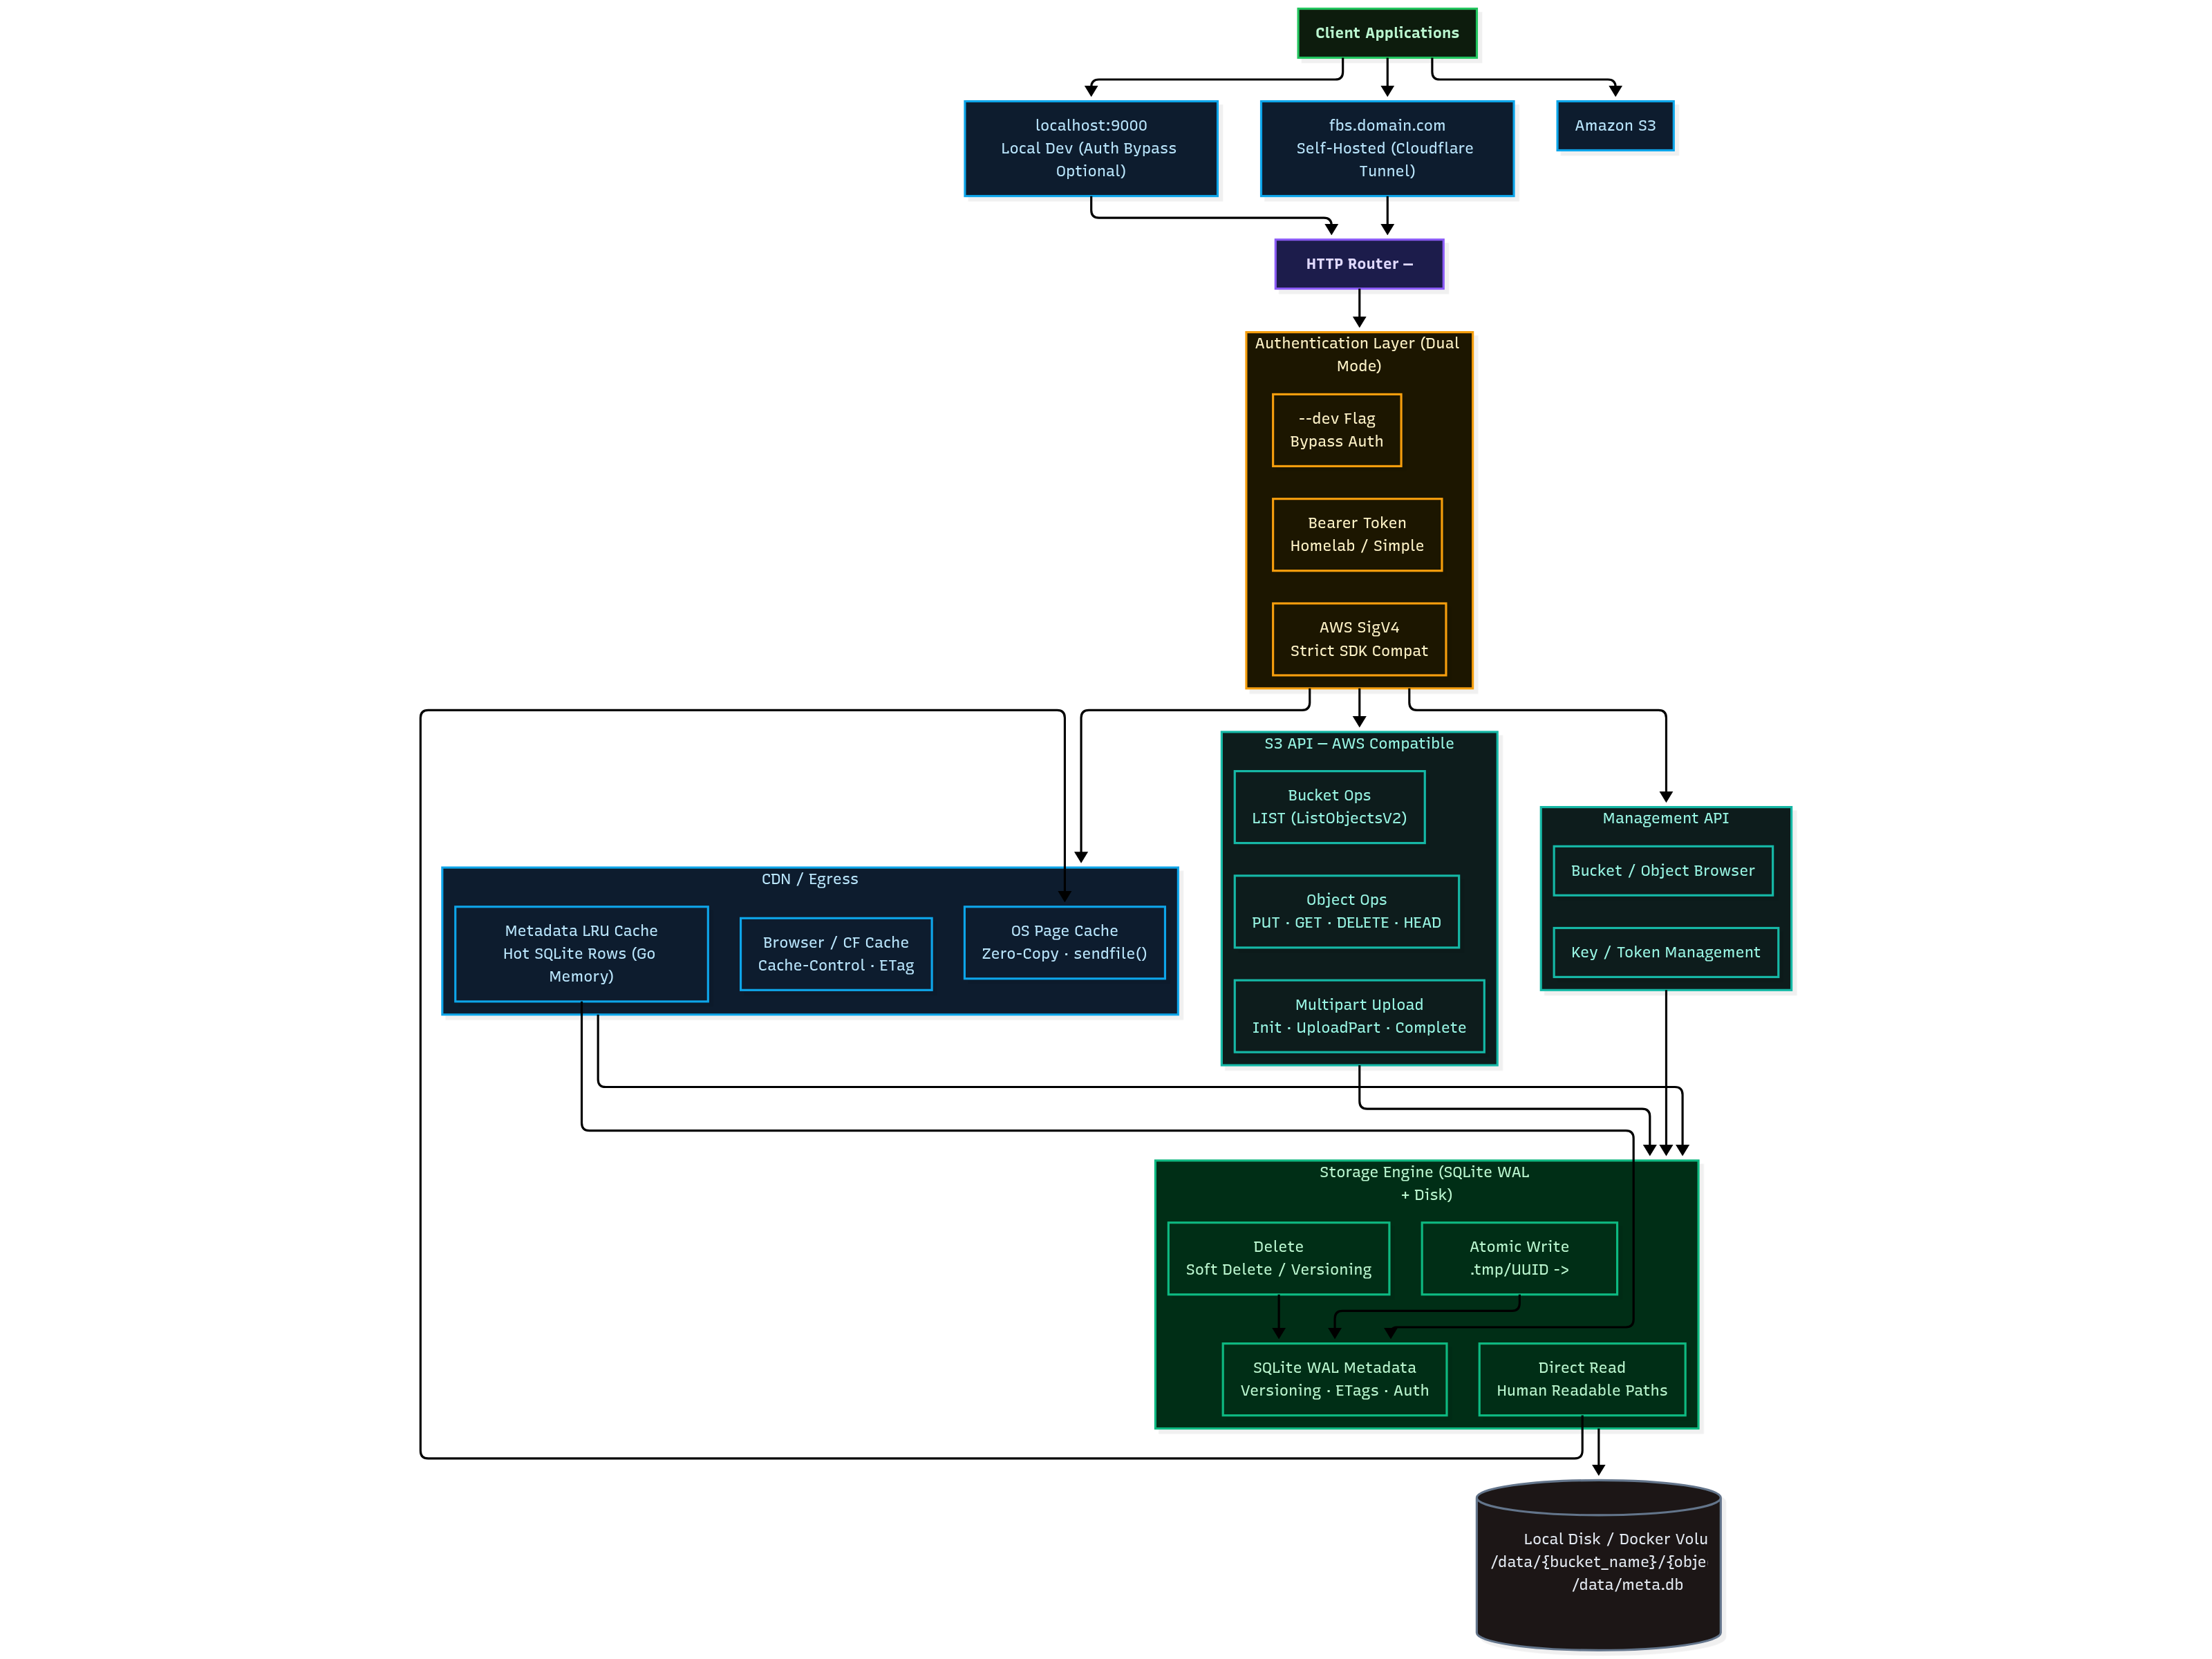
\includegraphics[width=1.1\textwidth]{flow.png}
\caption{System Architecture of the FBS: Fast Blob Storage}
\label{fig:architecture}
\end{figure}

The \textbf{Go backend} forms the core, handling all S3 operations and exposing two endpoint groups: the S3 API for object storage and the Management API for administration. The \texttt{chi} router handles routing with middleware for logging, panic recovery, and CORS. The S3 \texttt{GET} path uses a separate, minimal middleware chain to preserve the \texttt{io.ReaderFrom} interface on the response writer, enabling \texttt{sendfile()} zero-copy transfers; \texttt{http.ServeContent()} handles range requests, ETag, and Last-Modified in a single call.

The storage engine enforces a strict \textbf{data-before-metadata write order}: objects are first written to \texttt{.tmp/UUID}, atomically renamed to \texttt{/data/\{bucket\}/\{key\}}, and only then is metadata inserted into SQLite. This makes SQLite the single source of truth --- if a metadata row does not exist, the object does not exist. On server startup, a \textbf{reconciliation pass} purges incomplete files from \texttt{.tmp/} and removes any orphaned data files that lack a corresponding metadata row, ensuring self-healing after crashes. All object keys undergo \textbf{path sanitization}: keys containing traversal sequences (\texttt{../}), null bytes, or filesystem-invalid characters are rejected, and intermediate directories are created as needed for keys containing \texttt{/}.

Upload integrity is enforced through a \textbf{checksum validation pipeline}: \texttt{Content-MD5} and \texttt{x-amz-checksum-*} headers are verified on upload using a \texttt{TeeReader} that hashes data as it streams to disk, rejecting mismatches before metadata is committed. The computed MD5 is stored as the object's ETag. A \textbf{background goroutine} periodically purges multipart uploads older than a configurable TTL (default 24 hours), reclaiming disk space from abandoned uploads.

SQLite with WAL mode tracks metadata across four tables: \texttt{buckets}, \texttt{objects}, \texttt{multipart\_uploads}, and \texttt{keys}, tuned with \texttt{synchronous=NORMAL} and \texttt{busy\_timeout=5000} for optimal single-node write throughput.

The \textbf{web dashboard} (SvelteKit + TypeScript + TailwindCSS) connects via Management API, providing a metrics overview, file browser, and access key manager. The \textbf{terminal dashboard} (OpenTUI) offers a split-pane file explorer, object metadata views, and real-time metric charts with vim-style keyboard navigation.

Dual-mode authentication serves both SDK clients (AWS SigV4 signature verification) and simpler use cases (Bearer Token for dashboards and scripts). Bearer tokens are stored as \textbf{SHA-256 hashes} in SQLite --- raw tokens are returned to the user once at creation time and never persisted. A \texttt{--dev} flag bypasses authentication but is restricted to \texttt{localhost} binding only and logs a startup warning.

\section{Key Technologies and Tools}
\begin{table}[H]
\centering
\begin{tabular}{|p{4.5cm}|p{10cm}|}
\toprule
\textbf{Tool} & \textbf{Description} \\
\midrule
Go (Golang) & Backend server implementation; goroutines for concurrency, native HTTP performance \\
\midrule
chi Router & Lightweight HTTP routing with middleware support \\
\midrule
SQLite (WAL Mode) & Embedded metadata storage; WAL enables concurrent reads during writes \\
\midrule
HashiCorp LRU & In-memory cache for hot metadata queries and frequently accessed objects \\
\midrule
SvelteKit + TypeScript + TailwindCSS & Web dashboard; file-based routing, SSR, responsive UI \\
\midrule
OpenTUI & Terminal dashboard; declarative TUI components in TypeScript \\
\midrule
Docker & Backend containerization with volume mounts for persistent storage \\
\bottomrule
\end{tabular}
\end{table}

\section{V.E.T.S Justification}

\vspace{0.3cm}
\noindent \textbf{V - Viability}\\
The project is highly feasible within the available timeframe and resources. The Go backend compiles to a single static binary with no external runtime dependencies, deployable via a single command. SQLite requires no server process or database administration. The estimated memory footprint is under 50 MB for the backend and sub-100 MB per dashboard, making deployment viable on Raspberry Pi, low-end VPS, and container environments.

\vspace{0.5cm}
\noindent \textbf{E - Engineering Depth}\\
The project spans multiple engineering disciplines. The S3 API implementation requires deep understanding of AWS SigV4 signing (canonical request reconstruction, HMAC-SHA256), HTTP semantics, XML response formatting, and S3 error code conventions. The storage engine involves atomic file operations, directory structure management, path sanitization against traversal attacks, and a data-before-metadata write ordering with startup reconciliation to guarantee consistency between the filesystem and SQLite. Upload integrity is enforced through a TeeReader checksum pipeline validating Content-MD5 at wire speed. The SQLite layer demands schema design, WAL concurrency tuning (\texttt{synchronous=NORMAL}, \texttt{busy\_timeout}), and query optimization. Credential security uses SHA-256 token hashing rather than plaintext storage. Egress uses Linux \texttt{sendfile()} syscalls for zero-copy transfers, requiring careful middleware chain design to preserve the \texttt{io.ReaderFrom} interface on the response writer.

\vspace{0.5cm}
\noindent \textbf{T - Trend Alignment}\\
The project aligns with the growing self-hosted and homelab movement driven by privacy concerns, cost optimization, and desire for infrastructure control. It follows the cloud-native, API-first design philosophy that dominates modern distributed systems development. The TypeScript-unified stack across web and CLI tooling reflects the industry trend toward full-stack JavaScript/TypeScript ecosystems.

\vspace{0.5cm}
\noindent \textbf{S - Social / Industrial Impact}\\
Homelab enthusiasts gain an accessible, lightweight S3 target for home media servers and self-hosted application stacks. Small teams benefit from a cost-effective alternative to commercial cloud storage, eliminating per-GB egress charges while retaining S3 tooling compatibility. Educational institutions can use it as a hands-on platform for teaching distributed systems, cloud storage concepts, and API design.

\section{Expected Outcomes}
\begin{itemize}
\item A fully functional Go-based S3-compatible storage server as a drop-in replacement for AWS S3.
\item Complete S3 API compliance for object CRUD, bucket listing, and multipart uploads, validated against the official AWS SDK.
\item Dual authentication: AWS SigV4 verification passing official test suites, and Bearer Token auth (SHA-256 hashed storage) for dashboards.
\item Data integrity guarantees through data-before-metadata write ordering, startup reconciliation of orphaned files, upload checksum validation, and automated stale multipart cleanup.
\item Security hardening including object key path sanitization against directory traversal, hashed credential storage, and restricted development mode.
\item A decoupled Management API with RESTful JSON endpoints.
\item A SvelteKit web dashboard for graphical administration and file management.
\item An OpenTUI terminal dashboard for keyboard-driven CLI management.
\item Egress optimizations including zero-copy transfers via a dedicated minimal middleware chain, LRU metadata cache, and HTTP caching headers.
\end{itemize}

\section{Implementation Timeline}
\begin{table}[H]
\centering
\begin{tabular}{|p{2cm}|p{12.5cm}|}
\toprule
\textbf{Phase} & \textbf{Activity} \\
\midrule
Phase 1 & Problem analysis and requirement study (Core HTTP Server \& Routing, SQLite Metadata Layer, Disk Storage Engine) \\
\midrule
Phase 2 & System design and architecture (Auth Framework, Bearer Tokens, Basic S3 Object Operations) \\
\midrule
Phase 3 & Implementation and module development (AWS SigV4 Auth, Bucket Operations, Management API) \\
\midrule
Phase 4 & Testing and evaluation (Multipart Uploads, Egress Caching Optimizations, Building Web \& CLI Dashboards) \\
\midrule
Phase 5 & Documentation and final presentation (End-to-end integration, Bug Fixes, Docker setup, Release) \\
\bottomrule
\end{tabular}
\end{table}

\renewcommand{\bibname}{\centering \normalfont\Large\bfseries 9. References}
\begin{thebibliography}{99}

\bibitem{aws-s3}
Amazon Web Services, ``Amazon S3 API Reference [Online]. Available: \url{https://docs.aws.amazon.com/AmazonS3/latest/API/Welcome.html}

\bibitem{minio}
MinIO, Inc., ``MinIO Object Storage [Online]. Available: \url{https://min.io}

\bibitem{sigv4}
Amazon Web Services, ``Authenticating Requests: Using Query Parameters (AWS Signature Version 4) [Online]. Available: \url{https://docs.aws.amazon.com/AmazonS3/latest/API/sigv4-query-string-auth.html}

\bibitem{go}
The Go Authors, ``The Go Programming Language [Online]. Available: \url{https://go.dev}

\bibitem{chi}
Go-Chi, ``chi --- lightweight, idiomatic router for Go [Online]. Available: \url{https://github.com/go-chi/chi}

\bibitem{sqlite}
SQLite Consortium, ``Write-Ahead Logging [Online]. Available: \url{https://www.sqlite.org/wal.html}

\bibitem{sveltekit}
Svelte Team, ``SvelteKit [Online]. Available: \url{https://kit.svelte.dev}

\bibitem{opentui}
OpenTUI, ``Terminal UI Library for TypeScript [Online]. Available: \url{https://github.com/anomalyco/opentui}

\bibitem{sendfile}
Linux Kernel, ``sendfile(2) --- transfer data between file descriptors. [Online]. Available: \url{https://man7.org/linux/man-pages/man2/sendfile.2.html}

\bibitem{hashicorp-lru}
HashiCorp, ``golang-lru --- Golang LRU cache implementation [Online]. Available: \url{https://github.com/hashicorp/golang-lru}

\bibitem{garage}
Deuxfleurs, ``Garage --- An open-source distributed object storage service [Online]. Available: \url{https://garagehq.deuxfleurs.fr}

\end{thebibliography}

\end{document}